In the previous chapter, we showed that symbolic models are effective for environments with a stable interface, such as operating systems.
%
For interfaces with incomplete and unstable specifications, such as those of popular dynamic languages like Python and Ruby, the environment problem lends itself to a different approach.
%
In this chapeter, we present \chef, a symbolic execution platform for interpreted languages that relies on using the language interpreter as an ``executable language specification''.

\section{System Overview}

\begin{figure}
  \centering
  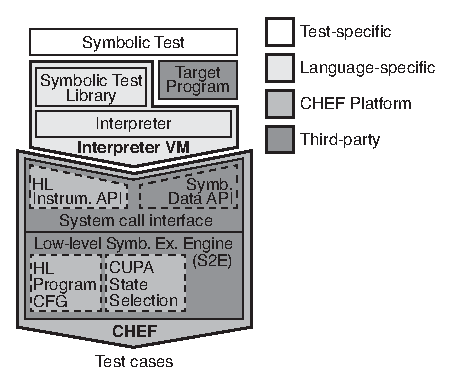
\includegraphics[width=0.8\textwidth]{figures/chef/system-arch}
  \caption{Overview of \chef's usage.}
  \label{fig:chef:overview}
\end{figure}

\chef is a platform for language-specific symbolic execution.
%
Provided with an interpreter environment, which acts as an executable language specification, it becomes a symbolic execution engine for the target language (see Figure~\ref{fig:xxx}).
%
The resulting engine can be used like a hand-written one, in particular for test case generation.  When fed with a target program and a symbolic test case (also called test driver or test specification in the literature), it outputs a set of concrete test cases, as shown in Figure~\ref{fig:chef:overview}.

\chef is built on top of the S2E analysis platform~\cite{s2eSystem}, which symbolically executes the interpreter environment \emph{at binary level}.
%
The interpreter environment is a virtual machine that bundles the interpreter, a testing library, the operating system, and other user programs.

The resulting engine is a correct symbolic execution engine for the target language \emph{as defined by the interpreter}.
%
It is fully precise and theoretically complete, i.e., it will not explore infeasible paths and will eventually explore all paths.\footnote{The usual limitations of symbolic execution engines apply: completeness holds only under the assumption that the constraint solver can reason about all generated path conditions, and it is understood that exhaustive exploration is usually impractical in finite time.}

\section{\chef's Architecture as Adapter Between Engine Interfaces}

\begin{figure}
  \centering
  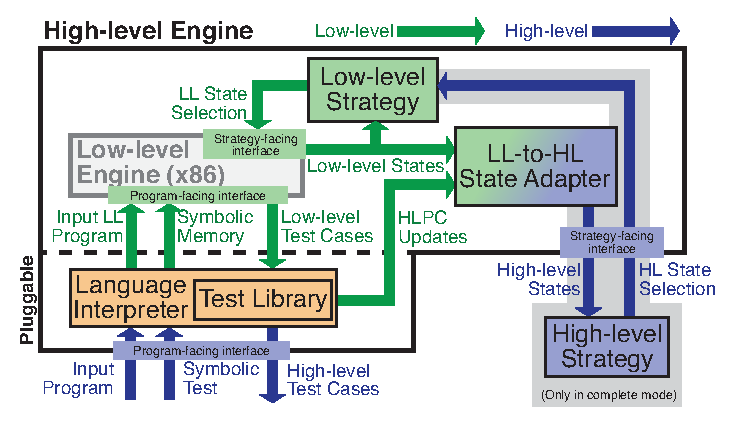
\includegraphics[width=0.8\textwidth]{figures/chef/iface-adapter}
  \caption{The architecture of \chef.}
  \label{fig:chef:arch}
\end{figure}

From a systems perspective, \chef acts as an adapter between two symbolic execution engine interfaces:
%
the internal \emph{low-level} binary engine, and the developer-facing \emph{high-level} engine interface.

Broadly speaking, the interface of a symbolic execution engine consists, on the one hand, of the part that receives the program and the test driver, and outputs test cases.
%
On the other hand, it also includes the communication interface with the execution strategy, i.e., the component that decides which of the available program states in the execution tree to be run next (see Section~\ref{sec:intro:symbex}).

Figure~\ref{fig:chef:arch} shows the architecture of \chef, which consists of a fixed part and a pluggable part.
%
The fixed part includes the low-level symbolic execution engine (S2E), its state selection strategy, and a state adapter, which converts low-level execution states in the interpreter to high-level execution states in the target program.
%
The pluggable part contains the language interpreter, responsible with providing the implicit semantics of the language.

The inner low-level symbolic execution engine operates with machine-level abstractions (the gray component in Figure~\ref{fig:chef:arch}).
%
It runs a binary program and marks memory bytes from its address space as symbolic inputs.  In return, it provides test cases consisting of concrete values for the marked bytes.
%
During symbolic execution, the low-level engine informs the low-level execution strategy of all states created in the execution tree, and the strategy decides which of them to execute next.

The outer interface exposes similar abstractions, but at the high level (the outer block in Figure~\ref{fig:chef:arch}).
%
The high-level engine runs an interpreted program and marks objects in the program state, such as strings and numbers, as symbolic inputs.  In return, the engine provides concrete object values as test cases.
%
Optionally, a high-level execution strategy decides which high-level states to prioritize.

In the following sections, we describe in detail the techniques \chef employs to fulfill its interface adapter role.

\section{From Low-level to High-level Symbolic Execution Trees}

The most important function of \chef is to pick the low-level execution paths in the interpreter that maximize its effectiveness as a high-level symbolic execution engine.
%
This is handled by \chef's fixed part, in a language- and interpreter-agnostic way.

The low-level path selection works as a feedback loop, as follows.
%
First, the low-level engine reports the progress of its states to a \emph{state adapter}, which maintains a high-level symbolic execution tree from the low-level states.
%
Second, the state adapeter sends the high-level execution tree updates to a pluggable high-level strategy, which decides the next high-level state to explore.
%
Finally, the selected high-level state is communicated to the low-level strategy, which takes it into account when selecting the next low-level state.

\paragraph{The State Adapter}

The high-level view consists of high-level states that form a high-level execution tree.

The high-level states are \emph{abstract}, as they only include a \emph{high-level program counter} (HLPC) and, optionally, a path condition.
%
The high-level program data is not exposed in a \chef state, as its semantics are language-dependent.  However, the program data is implicitly encoded in the low-level interpreter state.

The paths in the high-level tree envelop the paths in the low-level interpreter tree.

The state adapter groups the low-level paths that execute the same sequence of HLPCs.

The number of low-level paths mapping to the same high-level path can be very large.

\section{Trading Precision and Efficiency with State Completeness Models}

The state adapter has two modes of managing the high-level states: partial and complete.
%
The two modes are trade-offs between precision of controlling the high-level execution and performance.

The two modes differ with respect to the position the high-level state is allowed to be on the high-level path.

A high-level path can be divided in three segments, defined by the position of the \emph{low-level states} on it.

For each point on the high-level path, we define a path condition as the disjunction of the path conditions of all low-level states that have traversed the point.

We also define the cost of advancing a high-level state as the cost of exploring the low-level states underneath in order to advance the path segment.

\subsection{Partial High-level Execution States}

Under the partial model, a high-level state is allowed to be anywhere on the completed and partial segments.

Under the partial model, \chef cannot decide whether a high-level state would branch at the current HLPC.

The consequence of this property is that a high-level strategy cannot control the ordering of high-level paths.

However, the advantage of partial states is that they can progress efficiently, as only one low-level state needs to be advanced.

As a result, in practice, \chef takes full advantage of this property and always keeps the partial states on head of the path, guided by the leading low-level states.

\subsection{Complete High-level Execution States}

Under the complete model, a high-level state can only reside on the completed path segment.

Branch feasibility is decidable in the complete model, as the high-level path condition is complete.

As a result of branch feasibility, the symbolic execution engine has a choice over which high-level states to explore next.

However, advancing a high-level state is more expensive, as all low-level states on the path need to make progress.

\subsection{Choosing Between the Two Models}

\newcommand{\goodcolor}{\cellcolor{LimeGreen}}
\newcommand{\badcolor}{\cellcolor{Lavender}}

\begin{table}
  \centering
  \small
  \begin{tabular}{r c c}
    High-level State Model & \textbf{Partial} & \textbf{Complete}               \\
    \hline
    \noalign{\smallskip}
    Location (HLPC) & Complete and partial segments & Complete segments only    \\
    Path Condition  & Incomplete                    & Complete                  \\
    Strategies      & Only at low level             & Both high- and low-level  \\
    \noalign{\smallskip}
    \hline
    \noalign{\smallskip}
    Efficiency (state cost) & \goodcolor One low-level state   & \badcolor All low-level states      \\
    Precision       & \badcolor Low (no branch feasibility)   & \goodcolor Full control over states  \\
  \end{tabular}
  \caption{Comparing partial and complete high-level state models in \chef.}
  \label{tab:chef:hl-states}
\end{table}

Table~\ref{tab:chef:hl-states} summarizes the trade-offs between the partial and complete state models.

Both state models are useful for symbolic execution.

The partial state model works best for exploratory automated test case generation.

The precise state model is more appropriate for directed test case generation and exhaustive testing.

\section{Search Strategies in \chef}

Recall that the main goal of \chef was to prioritize the right low-level execution paths in the interpreter that maximize a high-level goal.

Partial and complete high-level state models lend themselves to different approaches.

As partial states do not offer a view into the available high-level states, the low-level strategy takes neutral decisions.
%
\chef uses CUPA (...)

In the complete state model, the state selection happens in two stages: a high-level strategy decides the next high-level state to prioritize, then the low-level strategy picks an appropriate low-level state for that.


\section{The Role of the Language Interpreter in Providing Semantics}

The input high-level program is bundled with the interpreter inside a virtual machine, and executed at the x86 level.

Symbolic tests set up the program and inject symbolic inputs, which consist of high-level objects, such as strings and integers.

The test library converts between the high-level objects and memory bytes, which is what the low-level engine understands.



%%%%%%%%%%%%%%%%%%%%



%%%%%%%%%%%%%%%%%%%%%%%%%%%%%%%%%%%%%%%%%%%%%%%%%%%%%%%%%%%%%%%%%%%%%%%%%%%%%%%%

\section{High-level Symbolic Execution}
\label{sec:chef:hlsymbex}

%% When executing the interpreter, \chef provides the abstraction of a symbolic execution engine that executes the target high-level program.
%% %
%% In this section, we present how \chef constructs the symbolic execution tree of the program from that of the interpreter (Section~\ref{sec:chef:ll2hl}) and how high-level symbolic execution states progress along this tree (Section~\ref{sec:chef:hlstates}).

\subsection{High-level States and Paths}

\chef's high-level symbolic execution interface 


%%%%%%%%%%%%%%%%%%%%%%%%%%

Recall that, in general, a symbolic execution state contains the current program counter, the path condition (the set of all branch conditions taken by the state), and the symbolic memory contents of the program.
%
The sequence of program counters of the state determines one path in the symbolic execution tree.

\chef's symbolic execution engine interface provides \emph{abstract} high-level states and paths, which encapsulate the low-level execution of the interpreter.
%
The states contain an abstract \emph{high-level program counter} (HLPC) and optionally, the path condition.
%
The high-level state memory is undefined in \chef, as its semantics are language-dependant.  However, the symbolic memory is implicitly encoded in the low-level interpreter state.

The concrete semantics of the HLPC depend on the language and the interpreter.
%
\chef treats HLPC values opaquely, with the only assumption that each statement in the program maps to exactly one HLPC.  The sequence of all HLPCs taken by a high-level state forms a path in the high-level symbolic execution tree.
%
Section~\ref{sec:xxx} presents concrete HLPC semantics for the most popular interpreters in use today.

\subsection{From Low-level to High-level Paths}
\label{sec:chef:ll2hl}

%% An interpreted program conceptually executes both on a high level---the level of the target language---and a low level---the level of the interpreter.
%% %
%% The low-level program path is the sequence of machine instructions from the interpreter binary, including the code for internal bookkeeping (e.g., details of reference counting and garbage collection).

%% Defining the high-level program path depends on the nature and semantics of the language.  In this thesis, we focus on imperative dynamic languages, such as Python and JavaScript.  An execution path in these languages consists of a sequence of statements in the program.  We uniquely identify each statement in the program by its ``high-level program counter'' (HLPC), which, for now, we refer to it as an abstract value.
%% %
%% We present in Section~\ref{sec:xxx} a concrete definition of HLPCs and methods from obtaining them during interpreter execution.

\chef constructs the high-level tree of execution paths by grouping the low-level paths generated by executing the interpreter in the low-level symbolic execution engine, as follows.
%
For each low-level path in the interpreter, \chef reconstructs the sequence of HLPCs it executes by observing the statements fetched and executed in the interpretation loop (Section~\ref{sec:xxx}).
%
The low-level paths that execute the same sequence of HLPCs map to the same high-level path.  Figure~\ref{fig:xxx} illustrates the relationship between the low- and high-level paths as the high-level tree enveloping the low-level one.

In practice, the number of low-level paths mapping to the same high-level path can be very large.  Their number increases roughly exponentially with the number of internal interpreter branches occurring along the high-level path, caused by implementation details, such as garbage collection or reference counting. \stefan{Maybe remove the reference to exponential growth, and give instead an example.}
%
To mitigate the path explosion along high-level paths, \chef employs state prioritization heuristics, which are discussed in Section~\ref{sec:xxx}.

%% Third, a high-level branch can occur \emph{at any point after} the low-level paths branches inside the interpreter.  This impacts the effectiveness of the heuristics aiming at discovering new high-level paths through the interpreter.
%% %
%% For example, the interpreter may implement a branching statement in two distinct steps: a comparison and a conditional jump.  In Figure~\ref{fig:xxx}, three low-level paths fork within the single HLPC location for \codebit{email.find}.  The low-level paths remain on the same high-level path until reaching the branching HLPC, where they diverge into two distinct high-level paths.  The relevant alternate low-level states for covering the distinct high-level paths thus were located away from the location of the code interpreting the high-level control flow statement.
%% %
%% The issue of pre-determining branches is present also when exploring regular code, but it is ubiquitous when exploring code on interpreters.


\subsection{Defining High-level Abstract States}
\label{sec:chef:hlstates}

%% This limitation makes it more difficult to build analyses that read the program state, including search selection strategies, such as the coverage-optimized strategy in \klee~\cite{klee}.
%% %
%% However, the high-level state remains implicitly encoded in the low-level interpreter state and can be accessed by executing code in the target language, by the interpreter runtime.  Therefore, a possible workaround is to split the analysis in a language-independent part, running as part of Chef, and a language-dependent part, written in the target language and running as an interrupt in the interpreter context, whenever it is needed.

Determining the positions of a high-level state on its high-level path is not as clear-cut.
%
The low-level states on the high-level path may reside at different points on the path, so there is no straightforward mapping from them to the high-level state.
%
Instead, \chef provides two modes of operation---\emph{partial-state} and \emph{complete-state}---corresponding to where the high-level states are allowed to be on their path.

%% The partial state mode allows \chef to explore high-level paths faster, by using only one low-level path for supporting the execution, at the expense of missing the information needed to precisely determine high-level branches and hence discover new high-level paths.
%% %
%% In contrast, in complete state mode, \chef can precisely reason about high-level branches and therefore provides the means to implement high-level state selection strategies.  However, this comes at the expense of a slower path exploration rate.
%% %
%% We next describe in more detail the two \chef operating modes.

Before defining the two modes, it is useful to divide each high-level path in three segments (Figure~\ref{fig:xxx}):
\begin{itemize}
\item \emph{completed}, where all the low-level execution paths have been traversed by their states,
\item \emph{partial}, where at least one low-level execution path has been traversed, and
\item \emph{undiscovered}, where no low-level path has yet been explored.
\end{itemize}

The leading low-level state of the high-level path defines the boundary between the partial and undiscovered segment, while the trailing state on the path defines the boundary between the completed and partial segment.

\subsubsection{Partial High-level States}

In partial high-level state mode (or ``partial state'', for short), the high-level state of a branch in the high-level tree is located at the HLPC of the leading low-level state on the high-level path (Figure~\ref{fig:xxx}).

A new high-level state is created for each new high-level path discovered, and the state progresses together with the leading low-level state.
%
This makes the execution efficient, once the path is discovered.

% However, the high-level state lacks a complete path condition.  The state cannot determine the feasibility of a branching point, because it lacks the complete knowledge of all paths.  For example, the find statement in figure XXX, ....

However, a partial state lacks a complete path condition (hence its name), as the entire set of low-level states are necessary to describe all possible executions on the path.
%
In particular, from a partial state, \chef cannot tell the feasibility of a branch.  More generally, it cannot tell whether a statement is branching at all (e.g., due to exceptions).

The consequence of this model is that the program execution at the high-level cannot be directly controlled.  \chef can only resort to picking a new low-level path and expecting that it will lead to a newly discovered high-level path.
%
In other words, the goal of the system becomes that of maximizing the high-level path yield for the set of low-level paths explored.
%
However, as executing low-level paths is efficient, in practice, a judicious state selection strategy can effectively discover significantly more high-level paths compared to naively choosing paths at random (Section~\ref{sec:xxx}).


\subsubsection{Complete High-level States}

In complete high-level state mode, a high-level state may be located anywhere on the completed segment of its path.
%
Since all low-level paths are explored, the interpreter behavior on the high-level path is completely known.  In particular, the feasibility of any branching point is completely decided.

A complete state has a well-defined path condition: it is the disjunction of all path conditions of the low-level states at the moment they entered the HLPC of the state.

The cost of advancing a complete high-level state is higher than that of a partial state.  To advance by one high-level statement, \emph{all} low-level states on the path need to explore the statement.
%
In contrast, a partial state can be avanced as long at one low-level state (the leading one) makes progress on the path.

In complete state mode, the high-level state prioritization is decoupled from the low-level state prioritization, as long as the high-level states stay within the completed segments.
%
This allows \chef to provide a pluggable \emph{high-level strategy} interface, which provides guidelines to the underlying low-level strategy to advance the low-level state execution only on the paths of interest.

\subsubsection{Comparing the Two State Models}

% Table~\ref{tab:xxx} summarizes the differences between the two models.  While partial states are faster to explore, they lack predictability and control.

% This is similar to fuzzing: concrete inputs may discover new paths, but from them alone you cannot tell in advance which path is going to be discovered next (if at all).

Partial mode is useful for exploratory testing.

Complete mode is useful when a precise goal must be attained (in particular, when the goal is expressed with respect to high-level path properties).


%%%%%%%%%%%%%%%%%%%%%%%%%%%%%%%%%%%%%%%%%%%%%%%%%%%%%%%%%%%%%%%%%%%%%%%%%%%%%%%%

\section{Path Prioritization in The Interpreter}
\label{sec:chef:strategies}

% Executing the interpreter naively won't be efficient.  A lot of the interpreter paths redundantly explore the same program paths.

% Path prioritization is done depending on the state completeness model used.

% Partial states don't have a high-level branch view, so a strategy can only resort to low-level information and information already available in the explored paths.  Such strategies are less flexible, as they cannot directly optimize for a high-level goal.

% Complete states have a high-level strategy.  This one can influence a lower-level strategy (tactic) optimized for reaching the goal of the high-level strategy.

\subsection{Class-Uniform Path Analysis}

Consider using symbolic execution for achieving statement coverage on a program containing a function with an input-dependent loop.  At each iteration, the loop forks one additional state (or exponentially many, if there are branches in the loop). A strategy that selects states to explore uniformly is therefore biased toward selecting more states from this function, at the expense of states in other functions that fork less but contribute equally to the statement coverage goal.

We reduce this bias by introducing Class-Uniform Path Analysis (\cupa).
%
The main idea is to group states into classes and then choose uniformly among classes instead of states.  For instance, in the above example, the class of each state could be its current function.  \cupa then first selects uniformly a function, then picks at random a state inside that function.  This way, functions generating many states are still selected with equal probability to others.

In general, \cupa organizes the state queue into a hierarchy of state subsets rooted at the entire state queue (see Figure~\ref{fig:cupa}).  The children of each subset partition the subset according to the \emph{state classification scheme} at their level.  A classification scheme is defined as a function $h: S \rightarrow C$, where $h(s)$ maps each state $s$ into a class value $c$.  States of the same parent with the same class value are sorted into the same child.
%
\begin{figure}
  \centering
  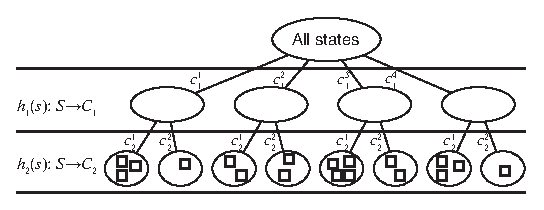
\includegraphics[width=3.2in]{figures/cupa/cupa}
  \caption{\cupa state partitioning.  Each level corresponds to a state classification scheme.  Child nodes partition the parent node according to the classification at their level.}
  \label{fig:cupa}
\end{figure}
%
\cupa selects a new state for exploration by performing a random descent in the classification tree, starting from the root.  When reaching a leaf, the strategy takes out a random state from the state set and returns it to the symbolic execution engine for exploration.  By default, all sibling classes on each level have equal probability of being picked, but they can be assigned weights if required.

A \cupa strategy is parameterized by the number $N$ of levels in the tree and a classification function $h_i$ for each level $i=1 \ldots N$.  \chef uses two instantiations of \cupa: one optimized for covering high-level paths (Section~\ref{sec:chef:cupa-paths}) and one for covering the high-level CFG, i.e., statements (Section~\ref{sec:chef:cupa-coverage}).

\subsection{Path-optimized CUPA}
\label{sec:chef:cupa-paths}

A low-level strategy unaware of the high-level program would be implicitly biased towards picking high-level instructions that fork more low-level states than others, such as string operations or native calls.
%
To mitigate this, we instantiate a two-level \cupa strategy using the following classes:
\begin{enumerate}
\item The location of the state in the high-level symbolic execution tree.  This is the occurrence of the state's high-level program counter (\hlpc) in the unfolded high-level CFG, referred to as the dynamic \hlpc.  We choose the dynamic \hlpc to give each high-level path reaching the \hlpc the same chance to fork and subsequently diverge.
\item The low-level x86 program counter of the state.  This classification reduces the selection bias of ``hot spots'' of path explosion within a single complex instruction, such as a native function call.
\end{enumerate}

\subsection{Coverage-optimized CUPA}
\label{sec:chef:cupa-coverage}

Based on a coverage-optimized strategy introduced by the \klee symbolic execution engine~\cite{klee}, we developed a \cupa instance that partitions states according to their minimum distance to branches leading to uncovered code.
%
Alas, dynamic language interpreters do not generally have a static CFG view of the program, so code that has not been covered yet is not accessible to the search strategy.  The high-level CFG of the target program is dynamically discovered along each execution path.  On this CFG, we employ heuristics that (1) identify the instruction opcodes that may branch, and (2)~weigh the state selection toward states that are closer to these potential branching points.

First, \chef identifies the branching opcodes by collecting all high-level instructions that terminate a basic block with an out-degree in the CFG of at least $2$ (i.e., cause branching in the control flow).   We then eliminate the 10\% least frequent opcodes, which correspond to exceptions or other rare control-flow events.
%
Second, \chef identifies the potential branching points as those instructions in the CFG that have a branching opcode (as previously identified) but currently only one successor.
%
Finally, \chef computes for each execution state the distance in the CFG to the closest such potential branching point.

Having computed this information, we instantiate a two-level \cupa strategy with the following classes:
\begin{enumerate}
\item The static \hlpc of the state in the high-level CFG.  On this level, each class is weighted by $\frac{1}{d}$, where $d$ is the distance in the inferred high-level CFG to the closest potential branching point, making states at locations close to a target more likely to be selected.
\item The state itself (so each partition has a single element).  On this level, the states are weighted by their \textit{fork weight}.
\end{enumerate}

Fork weight is computed by counting the number of consecutive forks at the same low-level program counter (i.e., at an input-dependent loop in machine code).  States $1, \ldots, n$ forking from the same path at the same location get weights $p^n, p^{n-1}, \ldots, 1$, where $p < 1$ de-emphasizes states forked earlier ($p = 0.75$ in our implementation).  The last state to fork at a certain location thus gets maximum weight, because alternating the last decision in a loop is often the quickest way to reach different program behavior (e.g., to satisfy a string equality check).


\subsection{Decoupling High-level From Low-Level Strategies}

% 


%%%%%%%%%%%%%%%%%%%%%%%%%%%%%%%%%%%%%%%%%%%%%%%%%%%%%%%%%%%%%%%%%%%%%%%%%%%%%%%%

\section{Interpreter Preparation}
\label{sec:chef:recipe}

To run an interpreter, \chef must be able to obtain the stream of high-level program counters (HLPCs) for each execution path.  For most interpreters of popular languages, \chef can perform this task fully automatically (Section~\ref{sec:chef:hlcf}), while providing a guest API for manual interpreter instrumentation as a fallback.

An optional step is to optimize the interpreter for symbolic execution (Section~\ref{sec:chef:optimizeforsymbex}).  \chef provides an API (Table~\ref{tab:api}) that will be explained along with its use.

Finally, we discuss the remaining work of building a language-specific testing API to the resulting engine (Section~\ref{sec:chef:testingAPI}).


\subsection{Automated High-level Control Flow Detection in Interpreters}
\label{sec:chef:hlcf}

In Section~\ref{sec:xxx}, we defined a high-level path as a sequence of statements identified by high-level program counters (HLPCs).  In this section, we present the concrete semantics of the HLPC and how \chef obtains it automatically from a running interpreter.

\begin{table}
\centering
\small
\begin{tabular}{| l | l | }
\hline
\textbf{API Call} & \textbf{Description} \\
\hline
\codebit{log\_pc(pc, opcode)} & Log the interpreter PC and opcode \\
\hline
\codebit{start\_symbolic()} & Start the symbolic execution \\
\codebit{end\_symbolic()} & Terminate the symbolic state \\
\hline
\codebit{make\_symbolic(buf)} & Make buffer symbolic \\
\codebit{concretize(buf)} & Concretize buffer of bytes \\
\codebit{upper\_bound(value)} & Get maximum value for expression\\
                              & on current path \\
\codebit{is\_symbolic(buf)} & Check if buffer is symbolic \\
\codebit{assume(expr)} & Assume constraint \\
\hline
\end{tabular}
\caption{The \chef API used by the interpreters running inside the S2E VM.}
\label{tab:api}
\end{table}

\begin{figure}
  \centering
  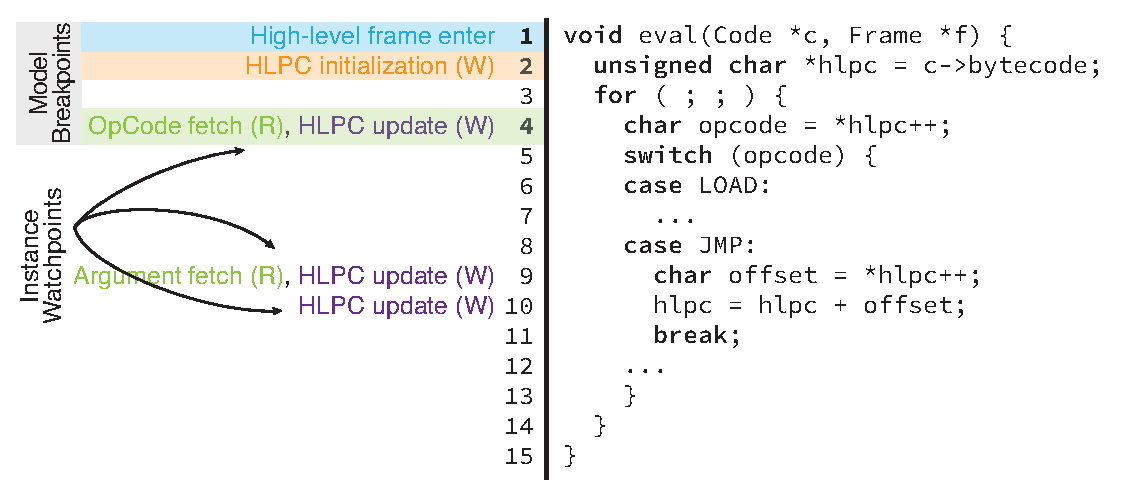
\includegraphics[width=0.8\textwidth]{figures/chef/interp-model}
  \caption{Structure of interpretation loop in most common interpreters.  Lines 1, 2, and 4 are three key HLPC points.  High-level control flow changes at Lines 4, 9, and 10 are detected at runtime by watchpoints on HLPC address identified at Line 2.}
  \label{fig:chef:interp-model}
\end{figure}

\paragraph{Standard Interpretation Model}

In general, obtaining the high-level program counter in a running interpreter is undecidable.
%
The boundaries between program statements are a high-level property of the language, and the separation may not reflect in the low-level implementation.  Even at the high level, statement boundaries may be ambiguous due to functional constructs, such as lambda functions and list comprehensions, or data definitions mixed with control flow, such as the class definitions in Python.

In practice, however, most interpreters follow a common structure that \emph{can be detected automatically}.
%
Instead of directly interpreting the source program, interpreters first compile it to an intermediate bytecode representation, which is interpreted instruction by instruction.  The bytecode is typically kept in per-function memory buffers.
%
When a function is called, the interpreter pushes a frame on its high-level stack, which contains a pointer variable to the next instruction in the function bytecode buffer.
%
An interpretation function receives the function bytecode and the stack frame, then executes the bytecode instructions one by one, while updating the HLPC variable of the frame (the right half of Figure~\ref{fig:chef:interp-model}).
%
We confirmed the generality of this approach by inspecting the source code of the most popular interpreters for Python, JavaScript (Mozilla's SpiderMonkey and WebKit's JavaScriptCore), Ruby, PHP, and Lua.

For these interpreters, we define the \chef high-level statements to be bytecode instructions, and their HLPC to be their address in the bytecode buffer.
%
As a result, to track the HLPC of the execution state, \chef monitors updates to the HLPC variable of the top high-level stack frame.

\paragraph{Tracking the HLPC Variable in the Interpreter}

To obtain the address of the top HLPC variable on the stack, \chef monitors three key locations in the interpretation function that summarize its HLPC update behavior:
%
(1) the address of the function itself, (2) the address of the statement that initializes the HLPC variable, and (3) the address of the statement that fetches the next opcode in the bytecode buffer.  The locations are highlighted on the left half of Figure~\ref{fig:chef:interp-model}.
%
\chef uses them as follows.

First, \chef maintains a stack of HLPC frames that track the interpreter's own high-level frames.
%
When the interpreter enters the interpretation function, \chef pushes a new HLPC frame on the current execution state.  A HLPC frame contains the address of the HLPC variable and its last value in the corresponding high-level frame of the interpreter.

Second, when the interpreter executes the HLPC initialization statement, \chef stores in the HLPC frame the memory address written to by the statement as the address of the HLPC variable.

Third, when the interpreter executes the opcode fetching statement, \chef marks the beginning of a new high-level statement at the address given by the current HLPC value.

During the execution of the interpretation function, \chef sets a watchpoint on the HLPC variable in the current frame.
%
When the variable is updated---e.g., when the next instruction is fetched, or after a branch or loop iteration---\chef correspondingly updates the HLPC value and the high-level symbolic execution tree, as needed.

\paragraph{Constructing the Interpreter HLPC Summary}

Before an interpreter is used for symbolic execution, \chef constructs its three-location HLPC summary.
%
The summary is constructed once for each interpreter binary.

First, \chef records all memory writes in the interpreter, when running a special developer-provided ``calibration'' script.
%
For each write, \chef records the interpreter location (x86 PC), the memory address, and the value written.

The role of the calibration script is to create HLPC update patterns that are recognizable among other memory writes.
%
The calibration script should run long enough that the HLPC patterns become clearly distinguishable.

To this end, \chef uses a linear sequence of instructions to create a linear HLPC update pattern.
%
We assume that the interpreter compiles a linear program (no branches) to a linear sequence of bytecode instructions.

After all memory writes are collected, \chef groups them by address and discards the groups whose values are not monotonically increasing.
%
Among the remaining groups, \chef discards those with fewer writes than the number of statements in the calibration program.  For this step, we assume that each statement corresponds to one or more bytecode instructions.
%
Finally, \chef discrads the groups whose write value deltas are larger than the size of a bytecode instruction.  We empirically determined an upper bound threshold of 1KB.

At the end, there should be exactly one remaining group, whose address refers to the HLPC variable of the frame of the recorded execution.

From the HLPC variable, \chef obtains the three-location summary.
%
The HLPC initialization location is the x86 PC of the first write operation in the remaining group.
%
The HLPC initialization location then leads to the address of the interpretation function, either by dynamically tracking the low-level program stack, or by using debug symbols in the interpreter binary.
%
Finally, the opcode fetch point corresponds to the first memory read of the HLPC variable, inside the interpretation function.

In case the calibration ends with no remaining memory write group, or more than one group remaining, the calibration fails.
%
This could happen, for instance, when the calibration is attempted on a non-conforming interpreter, or when the calibration script is too short.  To this end, we empirically determined that a 100-statement calibration script is sufficient for a successful calibration for all interpreters we tested.

\paragraph{Discussion}

In principle, defining program statements at an intermediate representation risks missing paths at the high-level.
%
This would happen, for instance, if the interpreter translated code with complex control flow to a linear bytecode sequence.
%
However, in our experience, we noticed that the translated bytecode follows closely the structure of the program.
%
In particular, interpreters perform little or no optimization on the bytecode.

\paragraph{Manually Annotating the High-level Program Counter}

When the interpreter structure diverges from our assumptions, \chef provides a fallback option of manually annotating the interpreter with the HLPC information (Figure~\ref{fig:xxx}).

\subsection{Interpreter Optimizations}
\label{sec:chef:optimzeforsymbex}

In order to maximize performance, interpreters make heavy use of special cases and sophisticated data structures.  Unfortunately, these features hurt the performance of symbolic execution by amplifying path explosion and increasing the complexity of symbolic formulas~\cite{overify}.

We identify a number of easy optimizations that preserve the interpretation semantics but significantly improve symbolic execution performance.  The optimizations use the \chef API in the last block of rows in Table~\ref{tab:api}.

\paragraph{Neutralizing Hash Functions}

Hash functions are especially common in interpreters, due to the internal use of hash tables for associative data structures (e.g., Python dictionaries or Lua tables).  However, they are generally a problem in symbolic execution: a symbolic value added to a hash table (a)~creates constraints that essentially ask the constraint solver to reverse a hash function, which is often hard, and (b)~causes the exploration to fork on each possible hash bucket the value could fall into.
%
A simple and effective optimization is to \emph{neutralize the hash function}, i.e., replace it with a degenerate one returning a single constant. This change honors the usual contracts for hash functions (equal objects have equal hashes) and will turn hash lookups into list traversals.

\paragraph{Avoiding Symbolic Pointers}

Input-dependent pointers (also referred to as symbolic pointers) may point to multiple locations in the program memory, so a pointer dereference operation would have to be resolved for each possible location.  In practice, symbolic execution engines deal with this situation in one of two ways:
%
(a)~fork the execution state for each possible concrete value the symbolic pointer can take; or
%
(b)~represent the dereference symbolically as a read operation from memory at a symbolic offset and let the constraint solver ``deal'' with it.
%
Both ways hurt symbolic execution, either by causing excessive path explosion or by burdening the constraint solver.

While there is no generic way to avoid symbolic pointers other than concretizing their values (the \codebit{concretize} API call) at the price of losing completeness, there are specific cases where they can be avoided.

First, \emph{the size of a buffer can be concretized} before allocation.  A symbolic size would most likely cause a symbolic pointer to be returned, since a memory allocator computes the location of a new block based on the requested size.  To avoid losing completeness, a symbolic execution-aware memory allocator can determine a (concrete) upper bound on the requested size and use that value for reserving space, while leaving the original size variable symbolic.  This way, memory accesses to the allocated block would not risk being out of bounds.  Figure~\ref{fig:sym-malloc} shows how the \chef API is used to wrap a call to the \codebit{malloc} function in the standard C library.

\begin{figure}
  \centering
  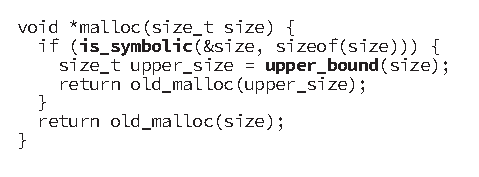
\includegraphics[width=2.6in]{figures/chef/mallocopt}
  \caption{Example of a symbolic execution-aware \codebit{malloc} function wrapper created using the \chef API.  If the allocation size is symbolic, the wrapper determines its upper bound and issues a concrete request to the underlying implementation.}
  \label{fig:sym-malloc}
\end{figure}

Second, \emph{caching and ``interning'' can be eliminated}.  Caching computed results and value interning (i.e., ensuring that a single copy of each possible value of a type is created) are common ways to improve the performance of interpreters.  Alas, when a particular value is computed, its location in memory becomes dependent on its value. If the value was already in the cache or in the interned store, it is returned from there, otherwise a new value is computed.  During symbolic execution, this logic becomes embedded in the value of the returned pointer, which becomes symbolic.  Disabling caching and interning may hurt the native performance of the program, but it can give a significant boost when running inside a symbolic execution engine.

\paragraph{Avoiding Fast Paths}

A common way to speed-up the native performance of a function is to handle different classes of inputs using faster specialized implementations (``fast paths'').  For example, a string comparison automatically returns false if the two strings have different lengths, without resorting to byte-wise comparison.

Fast paths may hurt symbolic execution because they cause symbolic branches in the code checking for the special input conditions.  \emph{Eliminating short-circuited returns} can reduce path explosion.  Instead of returning to the caller as soon as it produced an answer, the function continues running and stops on an input-independent condition.  For example, when comparing two strings of concrete length, a byte-wise string comparison would then traverse the entire string buffers in a single execution path, instead of returning after the first difference found.

\subsection{Testing API}
\label{sec:chef:testingAPI}

Programs to be tested can be fed symbolic inputs by marking input buffers with \codebit{make\_symbolic} and defining conditions over the input with the \codebit{assume} call, in accordance to the test specification.  Note that the buffer is a memory region of concrete bounds.  It is the job of the symbolic test library in the interpreter VM to convert from the language data structures (e.g., strings, integers) to the memory locations used to store the data in the interpreter implementation.


%%%%%%%%%%%%%%%%%%%%%%%%%%%%%%%%%%%%%%%%%%%%%%%%%%%%%%%%%%%%%%%%%%%%%%%%%%%%%%%%
%%%%%%%%%%%%%%%%%%%%%%%%%%%%%%%%%%%%%%%%%%%%%%%%%%%%%%%%%%%%%%%%%%%%%%%%%%%%%%%%

\iffalse
\section{Symbolically Executing the Interpreter}

Building a correct and complete symbolic execution engine for an interpreted language is generally harder than building one for a low-level language. 
%
Statements of interpreted languages can wrap complex operations that, in lower-level languages, would be implemented through libraries. For instance, Python strings are a built-in type offering more than 30 operations (such as \codebit{find}) as part of the language, implemented natively in the interpreter. 
%
Other language features that allow to inspect or even modify the code itself, i.e., runtime reflection, are even more tedious to implement and very hard to get right.

Finally, besides requiring an enormous initial effort to build a symbolic execution engine that fully supports them, dynamic languages also evolve fast. This implies constant, labor-intensive maintenance and co-evolution of the symbolic execution engine, if it is to keep up with the newest versions of the language.

Considering the difficulty of directly supporting interpreted languages, we resort to symbolically executing the interpreter itself, since it completely defines the semantics of the target language as a function of the semantics of the language the interpreter is implemented in.
%
After compiling the interpreter to a format supported by an existing symbolic execution engine, one can symbolically execute an interpreted program by symbolically executing the interpreter with the target program as argument.
%
However, even though in principle this direct approach yields a symbolic execution engine for the target language, it is impractical, due to the engine not being aware of the control flow of the interpreted program.

\paragraph{High- vs. Low-level Program Paths}

\begin{figure}
  \centering
  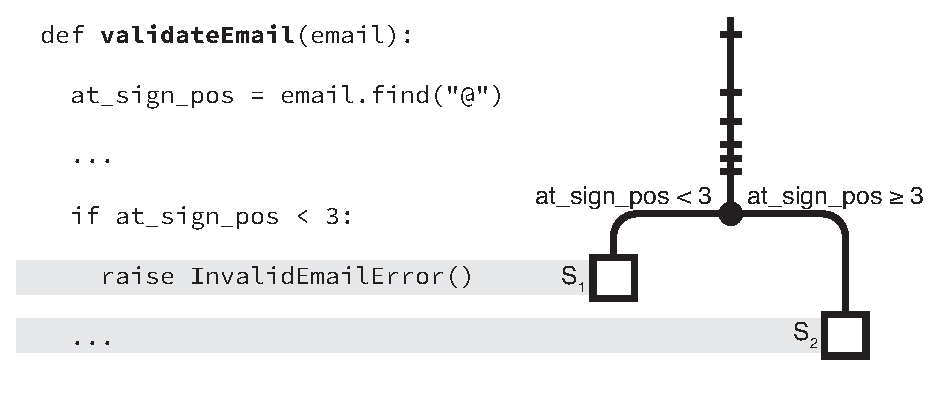
\includegraphics[width=2.2in]{figures/chef/running-example}
  \caption{Two examples of Python code that lead to path explosion when the interpreter running it is symbolically executed.}
  \label{fig:running-examples}
\end{figure}


An interpreted program conceptually executes both on a high level---the level of the target language---and a low level---the level of the interpreter.
%
A high-level program path is a sequence of values of the high-level program counter (\hlpc). Each \hlpc value corresponds to a program statement or bytecode instruction (both Python and Lua use intermediate bytecode).  Branches can occur explicitly at control flow statements, or implicitly through exceptions.
%
A low-level program path is a sequence of machine instructions from the interpreter binary, including its code for internal bookkeeping (e.g., details of reference counting and garbage collection).

Due to the additional implementation details, a single high-level path can map to multiple low-level paths.
%
Figure~\ref{fig:running-examples} shows two examples of Python code that have few high-level but many low-level paths. The \codebit{validateEmail} method has only two high-level paths, but its use of \codebit{string.find} leads to as many low-level paths as there can be characters in the \codebit{email} string.
%
The second example \codebit{average} may come as more of a surprise: even though it has just a single high-level path, symbolic execution can end up enumerating many low-level paths: Python uses arbitrary-precision integers, so the interpreter may have to iterate over digit vectors of arbitrary length, which can in principle spawn arbitrarily many paths.


\paragraph{Challenges for Search Strategies}
%
The search strategy of a low-level symbolic execution engine is oblivious to the high-level program structure of the target program, and it essentially just tries to cover the interpreter. This generally leads to covering the same high-level paths many times with multiple distinct low-level paths.
%
For instance, a high-level statement like \codebit{find} can lead to hundreds of alternate states, whereas a primitive integer comparison might just create a single one. Therefore, the low-level search strategy is likely to explore multiple ways for \codebit{find} to succeed or fail, without increasing high-level coverage, before eventually exploring the alternate outcome of the comparison.

\begin{figure}
  \centering
  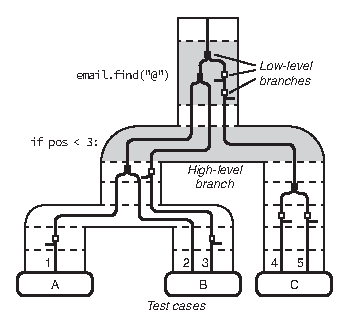
\includegraphics[width=2.8in]{figures/chef/hl-symbex}
  \caption{High-level execution tree (paths A, B, and C), as induced by its low-level execution paths (1--5) for the first running example in Figure~\ref{fig:running-examples}.  Dotted lines segment high-level execution paths into bytecode instructions.  One high-level path may correspond to multiple low-level paths explored.}
  \label{fig:hl-symbex}
\end{figure}

The key is to make the engine aware of the high-level interpreted program. By tracing the values of the \hlpc, the engine can construct a high-level control flow graph~(CFG) on the fly that can be be leveraged by the search strategy.

Alas, a strategy cannot straightforwardly determine future branching points in a high-level CFG: two low-level paths can fork from the same prefix \emph{before} their corresponding high-level paths do.  This can be due to having distinct bytecode instructions for comparisons and conditional jumps, or due to native library calls.  
%
In Figure~\ref{fig:hl-symbex}, three low-level paths fork within the single \hlpc location for \codebit{email.find}. The low-level paths remain on the same high-level path until reaching the branching \hlpc, where they diverge into two distinct high-level paths. The relevant alternate low-level states for covering the distinct high-level paths thus were located away from the location of the code interpreting the high-level control flow statement.
%
The issue of pre-determining branches is present also when exploring regular code, but it is ubiquitous when exploring code on interpreters.

\section{The \chef System}

We now present the architecture of \chef (Section~\ref{sec:chef:architecture}) and introduce \cupa, our state selection mechanism (Section~\ref{sec:chef:cupa}). We then describe \cupa optimized for exploring distinct high-level paths (Section~\ref{sec:chef:cupa-paths}) and optimized for high line coverage~(Section~\ref{sec:chef:cupa-coverage}).

\subsection{System Overview}
\label{sec:chef:architecture}

\chef is a platform for language-specific symbolic execution. Provided with an interpreter environment, which acts as an executable language specification, it becomes a symbolic execution engine for the target language (see Figure~\ref{fig:system-arch}).
%
The resulting engine can be used like a hand-written one, in particular for test case generation. When fed with a target program and a symbolic test case (also called test driver or test specification in the literature), it outputs a set of concrete test cases, as shown in Figure~\ref{fig:system-arch}.

\begin{figure}
  \centering
  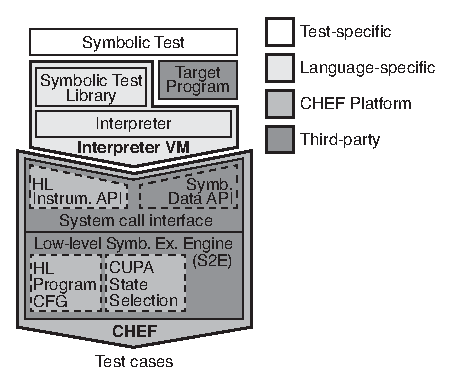
\includegraphics[width=2.6in]{figures/chef/system-arch}
  \caption{Schema of \chef's architecture.}
  \label{fig:system-arch}
\end{figure}

\chef is built on top of the S2E analysis platform~\cite{s2eSystem}. S2E symbolically executes a virtual machine containing the interpreter and a testing library at the level of machine code,  including the OS kernel, drivers, and user programs.  S2E provides an API that guest code can use to declare memory buffers as symbolic. Comparisons on symbolic values cause S2E to fork new paths, which are enqueued and explored following a search strategy.
%
\chef extends the S2E guest API with a high-level instruction instrumentation call (Section~\ref{sec:chef:exposehlpc}), invoked by interpreters to trace the currently executing high-level path.  The explored high-level paths are used to construct a high-level execution tree and a low-level to high-level mapping (i.e., the data structure shown in Figure~\ref{fig:hl-symbex}).  \chef uses a state selection strategy to maximize the ratio of high-level to low-level paths (Section~\ref{sec:chef:cupa}).

The resulting engine is a correct symbolic execution engine for the target language \textit{as defined by the interpreter}. It is fully precise and theoretically complete, i.e., it will not explore infeasible paths and will eventually explore all paths. The usual limitations of symbolic execution engines apply: completeness holds only under the assumption that the constraint solver can reason about all generated path conditions, and it is understood that exhaustive exploration is usually impossible in finite time.

%%%%%%%%%%%%%%%%%%%%%%%%%%%%%%%%%%%%%%%%%%%%%%%%%%%%%%%%%%%%%%%%%%%%%%%%%%%%%%%%

\subsection{Exposing the High-level Program Location}
\label{sec:chef:exposehlpc}

To reconstruct the high-level program paths and CFG, \chef needs to identify the high-level instructions executed on each low-level path.  \chef provides the \codebit{log\_pc(pc, opcode)} API call to the interpreter, which declares the current high-level program location and the type (opcode) of the next instruction.  A high-level instruction is executed in between two consecutive \codebit{log\_pc} calls.
%
Interpreters typically contain a main interpretation loop that \codebit{switch}-es over the type of the current instruction and invokes specific handlers.  The \codebit{log\_pc} call can be added conveniently at the head of the interpreter loop.

In our design, we make minimal assumptions about the language structure, so the \hlpc and opcode values are opaque; the \cupa strategies were designed accordingly.  Nonetheless, more specific versions of the system could add structure to the two values, e.g. provide a pair of function name and offset as \hlpc.  The additional information can be used by \chef to improve the exploration heuristics (e.g., by creating a \cupa class).

The granularity of \codebit{log\_pc} calls depends on the language structure.  \chef's correctness does not depend on the specific instrumentation pattern, but the more closely the reported \hlpc corresponds to statements in the target program, the more accurately \cupa can cluster states. In the extreme, if \codebit{log\_pc} is never invoked, \chef would see the entire program as a single high-level instruction and lose the advantage of \cupa clustering for \hlpcs.

\fi

%%% Local Variables: 
%%% mode: latex
%%% eval: (visual-line-mode)
%%% fill-column: 1000000
%%% TeX-master: "main"
%%% End:
